\documentclass[11pt]{article}

\usepackage{extras} % Se extras.sty
\usepackage{tikz}
\usepackage{graphicx}
\usepackage{epstopdf}

\usepackage{textgreek}
\usepackage{amsmath}


\usepackage{stringenc}
\usepackage{pdfescape}
\DeclareUnicodeCharacter{0308}{}



\begin{document}
\begin{titlepage}
\begin{center}

{\Large\bfseries TSEA56 - Kandidatprojekt i elektronik \\ LIPS Förstudie: Sensor}

\vspace{5em}

Version 0.1

\vspace{5em}
Grupp 4 \\
\begin{tabular}{rl}
Wasteson, Emil&\verb+emiwa068+
\\
Inge, Zimon&\verb+zimin415+
\\
\end{tabular}

\vspace{5em}
\today

\vspace{16em}
Status
\begin{longtable}{|l|l|l|} \hline

Granskad & - & - \\ \hline
Godkänd & - & - \\ \hline
 
\end{longtable}


\end{center}
\end{titlepage}

\pagebreak
\begin{center}

\section*{PROJEKTIDENTITET}
2016/VT, Undsättningsrobot Gr. 4

Linköpings tekniska högskola, ISY
\vspace{5em}
\begin{center}

\begin{tabular}{|l|l|l|l|} \hline
\textbf{Namn} & \textbf{Ansvar} & \textbf{Telefon} & \textbf{E-post}  \\ \hline 
Isak Strömberg (IS) & Projektledare & 073-980 38 50 & isast763@student.liu.se \\ \hline
Olle Hynén Ulfsjöö (OHU)& Dokumentansvarig & 070-072 91 84 & ollul666@student.liu.se \\ \hline
Emil Wasteson (EW) & Hårdvaruansvarig & 076-836 61 66 & emiwa068@student.liu.se \\ \hline
Elena Tronje (ET) & Mjukvaruansvarig & 072-276 92 93 & eletr654@student.liu.se \\ \hline
Zimon Inge (ZI)& Testansvarig & 070-171 35 18 & zimin415@student.liu.se \\ \hline
Lovisa Gustafsson (LG) & Leveransansvarig & 070-210 32 53 & lovgu777@student.liu.se \\ \hline
\end{tabular}

\end{center}

E-postlista för hela gruppen: isast763@student.liu.se

\vspace{5em}
Kund: ISY, Linköpings universitet \\
tel: 013-28 10 00, fax: 013-13 92 82 \\
Kontaktperson hos kund: Mattias Krysander \\
tel: 013-28 21 98, e-post: matkr@isy.liu.se \\

\vspace{5em}
Kursansvarig:  Tomas Svensson\\
tel: 013-28 13 68, e-post: tomass@isy.liu.se \\
Handledare: Peter Johansson \\
tel: 013-28 13 45, e-post: peter.a.johansson@liu.se
\end{center}
\pagebreak

\tableofcontents

\pagebreak
\section*{Dokumenthistorik}
\begin{table}[h]
\begin{tabular}{|l|l|l|l|l|} \hline

\textbf{Version} & \textbf{Datum} & \textbf{Utförda förändringar} & \textbf{Utförda av} & \textbf{Granskad} \\ \hline
0.1 & 2016/03/03 &  Första utkastet & Grupp 4 & ZI \\ \hline
\end{tabular}
\end{table}

\pagebreak
\pagenumbering{arabic}

\begin{flushleft}

\section{Inledning}
I dagsläget finns det en mängd olika sensorer, alla med för- respektive nackdelar. Vilken sensor som är bäst beror ofta på vilket syfte som ska uppfyllas och vilka resurser som finns att tillgå. Att en undsättningsrobot som ska hitta nödställda har sensorer som gör det enkelt att identifiera sitt mål är en fråga om liv och död. Därav finns det ett stort behov av att öka kunskapen om sensorer, samt dess möjligheter och begränsningar.


\section{Problemformulering}

\subsection{Syfte}
Syftet med denna rapport är att undersöka vilka sensorer som är relevanta för undsättningsroboten i sitt uppdrag. Syftet är fortsättningsvis att redogöra för en implementation av de sensorer som finnes intressanta för undsättningsrobotens ändamål.


\subsection{Frågeställningar}
Nedan följer de huvudsakliga frågeställningar vilka har för avsikt att behandlas i denna rapport:



\begin{itemize}

	\item	 Vilka sensorer finns det som stöd för att roboten ska kunna utföra sitt uppdrag? Hur fungerar dessa? Finns det olika typer?
	\item Vilka sensorer är lämpliga att använda till projektet?
	\item Hur kan dessa implementeras? 

\end{itemize}


\pagebreak
\section{Kunskapsbas}
För att kunna avgöra vilka sensorer som är ändamålsenliga för en undsättningsrobotot så krävs en redogörelse av vad som finns att tillgå. I följande avsnitt följer således en beskrivning av olika typer av sensorer.

\subsection{Kapacitiv sensor}
En kapacitiv sensor är en sensor som använder sig av kapacitans (C) för att identifiera ett önskat material. Sensorn består av en platta med arean A och kan detektera alla objekt som har en relativ kapacivitet som skiljer sig från luft, bland annat plast, olika metaller, vätskor och hud. Det finns olika typer av kapacativa sensorer, en del kräver kontakt mellan sensorn och ett objekt medan andra har högre känslighet och kan känna av kapacitansändringar på avstånd upp till 70 cm. När avståndet (d) mellan objektet och en sensorn minskar så ökar kapacitansen enligt ekvation \ref{kapacitiv}, där er är en konstant som beror av materialets relativa kapacivitet och eo är en permitiviteten i luften.\cite{website:capacative}


\begin{equation}\label{kapacitiv}
	\textrm{C} = \frac {e_{r} \times e_{o} \times A}{d}						
\end{equation}

I figur \ref{capacative} illustreras hur kapacitansen ändras när objektet (fingret) närmar sig sensorn och hur kapacitansändringen med hjälp av en AD-omvandlare görs om till en digital signal. 

\begin{figure}[htbp]
	\centering
	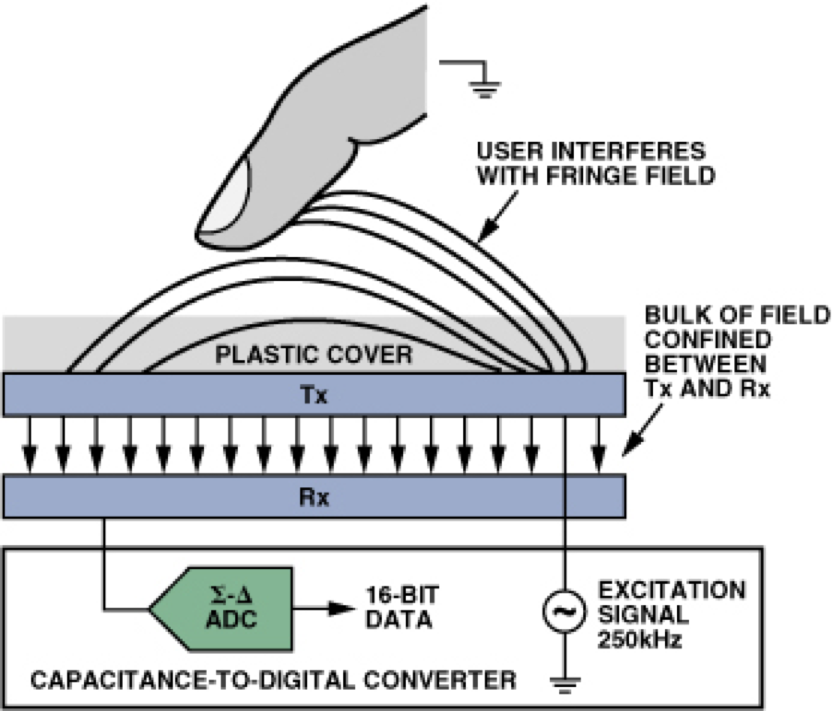
\includegraphics[scale=0.4]{Images/capacative}
	\caption{Ett fingers påverkan på kapacitans \label{capacative}}
\end{figure}

En kapacitiv sensor har många fördelar när ett objekt ska detekteras. Det som utmärker denna typen av sensor mest jämfört med övriga detektorer är att den kan detektera de flesta typer av objekt, alltfrån metaller och plast till hud och vatten. Det gör att samma sensor kan användas i flera typer av projekt och miljöer. Sensor behöver dock komma nära objekten som ska detekteras, vilket innebär att en bra uppfattning om var objektet krävs innan avsökning påbörjas. \cite{website:capacative}

%Förhållandet mellan kapacitans och spänning visas i figur 2.

%\begin{figure}[htbp]
%	\centering
%	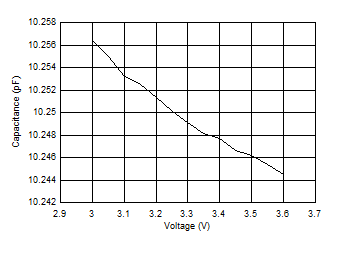
\includegraphics[scale=0.8]{Images/capacitance_voltage}
%	\caption{Förhållande mellan analog spänning och kapacitans \label{capacitance_voltage}}
%\end{figure}

\subsection{Ultraljudssensorer}
För att mäta avstånd till objekt kan en ultraljudssensor användas. Den skickar ut en puls av ljud, utanför det intervall människan kan uppfatta, för att sedan invänta ett eventuellt eko. Om inget eko detekteras finns det inget objekt inom sensorns avkänningsområde i den riktning som ljudpulsen skickades ut i. Uppfattas däremot ett eko registrerar sensorn hur lång tid (t) det tog för ljudet att studsa tillbaka och kan, eftersom ljudhastigheten (vluft) i luft är känd, utifrån det enligt ekvation \ref{ultra} räkna ut avståndet (s) till det objekt som gav upphov till ekot. 

\begin{equation}\label{ultra}
	\textrm{s} = v_{luft} \times t 				
\end{equation}

En ultraljudssensor passar bra i miljöer med skiftande omgivning. Den påverkas inte av vilka färger eller material som ljudvågorna studsar emot och den kan användas problemfritt i dammiga och smutsiga miljöer. Att mäta avstånd till små objekt på stora avstånd är inte heller någon begränsning då ljudvågorna breder ut sig på ett stabilt sätt.

Miljöer som begränsar ultralljudssensorer är höga tryck, vakuum och hög värme, men den största nackdelen att sensorn agerar förhållandevis långsamt. Ljudet utbereder sig med 340 m/s i luft, vilket gör att sensorn tar lbetydligt längre tid på sig att förmedla ett avstånd jämfört med sensorer som arbetar med ljus har en mycket högre hastighet. 

\subsection{Ljussensor}
En ljussensor (även kallad fotocell) består av en högresistiv halvledare vilken absorberar fotoner. Baserat på mängden fotoner sensorn absorberar och frekvensen på dessa så ges det halvledande materialets bundna elektroner tillräckligt med energi för att göra en förflyttning till ledningsbandet. De fria elektronerna medför sedermera att elektrisitet leds,  vilket i sin tur resulterar i att variaritioner i ljussensorns motstånd. Detta innebär att motståndet hos en ljussensor är högt i mörker, för att sedan minska i ljusare miljöer. \cite{612896}

Ljussensorn omvandlar följaktligen infallande ljus till elektrisk ström där strömstyrkan varierar beroende ljusets styrka. Av denna anledning så är en ljussensor användbar vid detektering av konstraster på exempelvis en yta.  \cite{612896}

En reflektorfotocell är en typ av ljussensor som, liksom ljussensorn, detekterar förändringar i ljusintensiteten. Det typiska i reflektorfotocellen är dock att den  består av en ljuskälla, en motagare, en signalkonverterare och slutligen en förstärkare. \cite{website:automation}


\subsection{IR-sensor}
En IR-sensor är en tillämpning av en ljussensor som endast registrerar önskade våglängder i det infraröda spektrumet. I figur \ref{Laser} illustreras hur en sensor, med hjälp av en LED-lampa som sänder ut strålning med samma våglängd som den sensorn uppfattar, kan avgöra om ett det finns ett objekt i sensorns riktning. Detekteras reflekterad strålning betyder det att ett föremål finns i sensorns riktning.  \cite{website:cmu}

\begin{figure}[htbp]
	\centering
	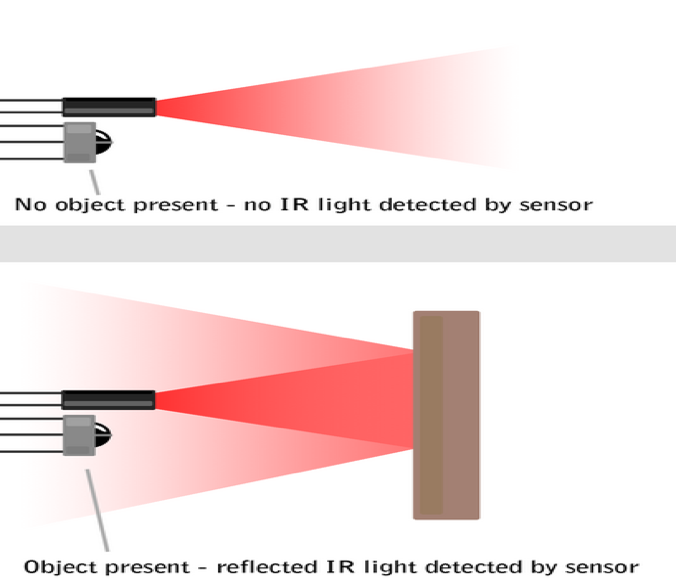
\includegraphics[scale=0.4]{Images/Laser}
	\caption{Illustration av lasersensor \label{Laser}}
\end{figure}

\pagebreak
Vissa IR-sensorer går även att använda som vinkelmätningssensor, genom att sensorn mäter vinkeln av det reflekterade ljuset som strålningen av LED-lampan ger upphov till. Detta illustreras nedan i figur \ref{laser_angle}. Vinkelmätning ställer emellertid högre krav på sensorn, eftersom strålningen som sänds ut från sensorn behöver vara skarpare.

\begin{figure}[htbp]
	\centering
	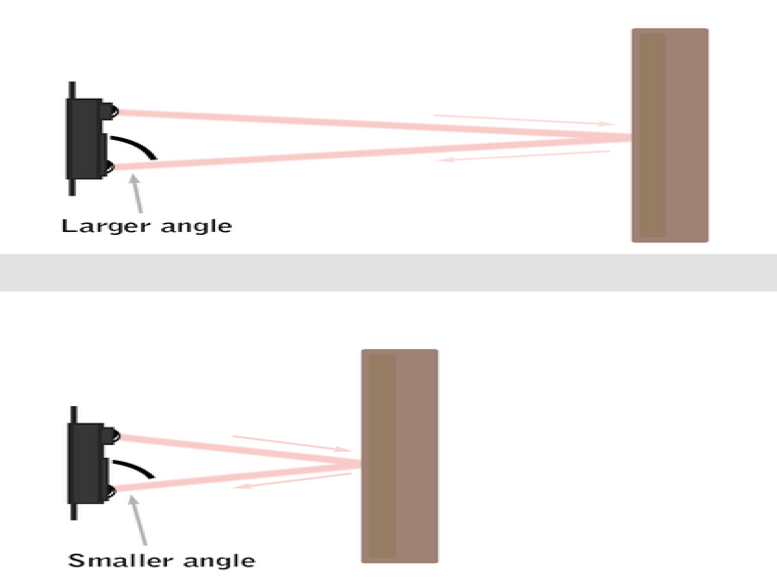
\includegraphics[scale=0.4]{Images/laser_angle}
	\caption{Vinkelmätning med lasersensor \label{laser_angle}}
\end{figure}

Ytterligare en möjlighet med en IR-sensor är att mäta hur ljusskillnader. Eftersom ljusa objekt reflekterar mer ljus än vad mörka gör kan sensorn reagera på reflektioner mot ett ljust objekt, men inte mot ett mörkt. \cite{website:cmu}

\subsection{Lasersensor}
Det finns olika typer av lasersensorer som använder olika tekniker foch har olika funktioner. En typ är den avståndsmätande elektrooptiska sensorn som sänder ut en laser stråle och mäter hur lång tid (t) det tar innan den reflekteras och detekteras av sensorn. Avståndet (D) är räknas fram enligt ekvation \ref{laser_eq}, där c står för ljusets hastighet i luft. \cite{website:mti}


\begin{equation}\label{laser_eq}
	\textrm{D} = \frac {c \times t}{2}						
\end{equation}

En annan typ av lasersensor är den triangulerade sensorn. De är mer komplex och kan mäta avstånd på ett mer precist sätt än den elektrooptiska. \cite{website:mti}

\subsection{Gyroskop}
För att mäta hur mycket rotation som sker gentemot omgivningen kan ett gyroskop användas. Genom att mäta vinkelhastigheten på rotationen (\textomega) kan storleken på rotationen (\straightphi) uppskattas genom integrering, enligt ekvation \ref{gyro}, där t står för tiden som rotationen har pågått. (3)

\begin{equation}\label{gyro}
	\phi = \int_{t}^{ }\omega dt 						
\end{equation}



%https://docs.isy.liu.se/pub/VanHeden/DataSheets/MPU-6050.pdf (4)

%http://www.mtiinstruments.com/pdf/appnotes/lasersensor.pdf (1)


\pagebreak
\section{Fallet undsättningsrobot}
De flesta har både fördelar och nackdelar. En del är mer precisa men dyra och komplicerade, medan andra är billiga och enkla men brister i kvalitet. I vissa fall är även designen viktig och ställer krav på de sensorer som används. I följande kapitel beskrivs vilka sensorer som passar för en undsättningsrobot. 

\subsection{Avståndssensor}
Det finns flera olika sensorer som klarar av att mäta avstånd till omgivande objekt. Här följer en beskrivning vilken typ av sensor som passar bäst till just en undsättningsrobot. 

\subsubsection{SRF04} %%ULTRALJUD
Ultraljudssensorn SRF04 mäter avstånd mellan 3 cm och 3 meter med hjälp av ultraljud. Den har en detektionskon på ca 30 grader, vilket gör att den kan upptäcka objekt trots att ekot inte studsar optimalt (vinkelrätt) mot ett objekt och den implementeras enkelt med en I\textsuperscript{2}C-buss. \cite{Devantech}

\subsubsection{GP2D120} %IR-SENSOR
IR-sensorn GP2D120 är en enkelt utformad sensor som tillverkas för att precisionsmäta avstånd på kortare avstånd, typiskt 4-30 cm. Att mätintervallet är jämförelsevis litet är en begränsning, men det gör samtidigt att kvaliteten av mätningar inom intevallet kan göras mer precist. 

För att kunna reglera på ett önskat sätt behöver roboten veta hur den förhåller sig i förhållande till sidoväggarna. Eftersom roboten ska kunna köra i mitten av korridorer med cirka 40 centimeters bredd och roboten själv är ca 20 cm bred, kommer ett avstånd mellan sidoväggarna och roboten på 10 cm vara önskvärt. För detta är IR-sensorn \verb+GP2D120+ bra, eftersom den precist kan mäta avstånd till objekt som befinner sig på ungefär 10-20 cm avstånd.

Mätandet av avstånd sker genom att IR-ljus med en viss våglängd skickas ut från sensorn, reflekteras mot väggarna för att sedan detekteras av sensorn. Genom att mäta den vinkel reflektionen sker med kan avståndet till väggen bedömas. \verb+GP2D120+ är relativt enkel och har enbart två ingångar som ska kopplas till en 5 volts strömkälla, respektive en jord.  Utsignalen är analog i form av spänning och på grund av mängden högfrekvent brus i signalen måste den lågpassfiltreras.

En svaghet hos sensorn är att den enbart kan användas inom ett litet intervall, vilket gör den till ett dåligt alternativ i en osäker omgivning eller där avstånd som ska mätas inte inkluderas i intervallet. Sensorn är även känslig för högfrekvent brus, vilket ofta existerar i omgivningen. Detta kan dock förebyggas genom att ansvända sig av lågpassfilter. 

\subsubsection{LIDAR-Lite v2}
Lidar-Lite v2 är en kraftfull lasersensor av begränsad storlek med ett flertal funktioner, till exempel avstånds- och hastighetsmätning av objekt. Den har en räckvidd på ca 40 meter med en felmarignal på på 0,025 meter och klarar även av att mäta signalstyrka på detta avstånd. \cite{Lidar}

%https://docs.isy.liu.se/pub/VanHeden/DataSheets/lidarlite2DS.pdf (2)
Denna lasersensor kan mäta avstånd till objekt med hög precision. Eftersom laser rör sig med ljusets hastighet och sensorn kan implementeras med avbrottshantering så sker mätningarna snabbt. Det är en stor fördel om flera sensorer delar på samma processor, eftersom endast en operation kan ske i taget. LIDAR-lite är mer avancerad och därmed dyrare än till exempel GP2D120, vilket gör att den inte bör användas om hög kvalitet efterfrågas. På en undsättningsrobot kan sensorn användas för att mäta avstånd frammåt till nästa objekt. Den kan även fästas på ett servo och kan på så sätt scanna av 360 grader av ett rum. \cite{Lidar}

Med hjälp av pulsbreddsmodulering kan förhållandet mellan en hög signal (en etta) och en låg signal (en nolla) bestämmas. Utifrån denna kvot kan sensorn kalibreras och en förhållande mellan en kvot och ett avstånd kan tas fram. \cite{Lidar}

\subsection{Detektering av mål}
Att identifiera objekt kan göras med hjälp av flera olika tekniker och sensorer, som alla har sina fördelar och nackdelar. I detta avsnitt följer en beskrivning av hur olika sensorer passar för detektering av ett mål på en undsättningsrobot.


\subsubsection{FDC1004} %KAPACITIV SENSOR
En sensor som inte kräver kontakt är FDC1004. Det kan implementeras med hjälp av en I\textsuperscript{2}C-buss och kan känna igen olika typer av material. \cite{Texas}, \cite{Texas2}

\subsubsection{IRM-8601S} %IR-Detektor
IR-detektorn \verb+IRM-8601-S+ används för att identifiera en källa som sänder ut IR-signaler. Utformandet av sensorn är relativt enkel med tre ingångar, en som kopplas till en 5V spänningskälla och en som ansluts till jord.

Denna IR-sensor är en enkelt utformad detektor känner av ljus i det infraröda spektrat. I och med att den är så pass enkelt utformad med begränsat användningsområde är den också relativt billig.  

\subsubsection{SFH300} %IR-SENSOR
SFH300 är en fotodiod med hög linjäritet som kan detektera våglängder i intervallet mellan 420 nm till 1130 nm. Detta betyder att denna fotodiod, utöver för ögat synligt ljus, även kan detektera infraröda våglängder. SFH300 leverar en analog spänning som utsignal, vilket innebär att en AD-omvandling är nödvändig innan en digital signal kan processeras. \cite{Osram}

Precis som IRM-8601S detekterar SFH300 vågor inom ett visst intervall, 420 nm till 1130 nm. Detta intervall inkluderar synligt ljus och även IR-vågor. Den kan alltså användas på ett bredare plan än IRM-8601S, vilket kan vara nödvändigt då det är säkert vad det är som ska detekteras. \cite{Osram}

\subsubsection{BPX43-3}
Liksom SFH300 så är även Siemens BPX43-3 även fotodiod som kan detektera infraröda våglängder. Idealt våglängdsintervall för denna fotodiolid ligger mellan 450 nm och 1100nm. Utsignalen är genereras i form av spänning, varför AD-omvandling krävs för processera utsignalen. Utspänningen ska emellertid vara mycket i linjär i förhållande till ljusstyrkan som dioden får som insignal. \cite{siemens}

\subsection{Vinkelhastighetsmätning}

\subsubsection{MPU-6050}
 MPU-6050 är en sensor som består av 3 gyroskop, 3 accelerometrar och en AD-omvandlare för varje enhet. För att kunna vara så exakt som möjligt i beräkningarna, både vid långsamma och snabba rörelser, kan användaren själv ställa in vilka intervall gyrot och accelerometern ska fokusera på. Sensorn kan kommunicera via ett I\textsuperscript{2}C-buss-interface. (4)

\subsubsection{MLX90609}
Sensorn MLX90609 är ett exempel på en sensor som består av ett gyroskop med uppgift att avgöra ett föremåls momentana vinkelhastighet. Sensorn kommicerar vinkelhastigheten i form av ett bitmönster via ett SPI-interface (Serial Peripheral Interface) till en masterenhet (anledningen till att den externa enheten väljs till master beror på att MLX90609 är förprogrammerad att alltid agera slav vid kommunikation till externa enheter). \cite{Melexis}

\subsection{Övriga funktioner}
% - MPU-6050


\pagebreak
\section{Resultat och slutsatser}
text

\pagebreak
\addcontentsline{toc}{section}{Referenser}




\pagebreak
\appendix
\section{First Appendix}

\end{flushleft}

\bibliographystyle{ieeetran}
\bibliography{references}
\end{document}
